%Correct the file name.
%X: book number
%Y: part number
%ZZZ: page number in three digits. So page 3 would be 003.

\documentclass[11pt]{amsbook}

\usepackage{../HBSuerDemir}	% ------------------------


\begin{document}

% ++++++++++++++++++++++++++++++++++++++
\hPage{018}
% ++++++++++++++++++++++++++++++++++++++
\noindent(j) Let $A$ be a nonempty set and let $B$ be fixed subset of $A$. For any $a$ in $A$, we put
$$x_{\!_B} = \begin{cases} 0 \text{ if }a \notin B, \\
 1\text{ if }a \in B.\end{cases}$$
Then $x_{\!_ B}$ is a function from $A$ into $ \hPairingCurly{0,1} $. It is called the \hDefined{characteristic function} of $B$. Here we wrote the function on the left.\\\\

\noindent(k) For any $x \in \hSoR$, we put
$$f(x) = \begin{cases} 0 \text{ if }x\text{  is irrational},\\
 1\text{ if }x\text{ is rational}.\end{cases}$$
Then $f$ is a function from $\hSoR$ into $\hSoR$. In fact, $f$ is the characteristic function of the set of rational numbers. The image of some $x$ is not known. For instance, it is not known whether Euler's constant $\gamma$ is rational or not. Nevertheless, $f$ is a genuine function. This example is due to L. Dirichlet (1805-1859). \\\\

\noindent(l) Let $A$ be a nonempty set and let $\sim$ be an equivalence relation on $A$. Let $A/\sim$ be the set of equivalence classes under $\sim$. Then 
\begin{align*}
v: A &\rightarrow A/\sim \\
a&\rightarrow  \hPairingBraket{a}\\
\end{align*}
is a mapping from $A$ into $A/\sim$ . It is called the \hDefined{natural mapping} or the \hDefined{canonical mapping from $A$ into $A/\sim$}.
\begin{defn}
Let $f: A\rightarrow B$ and $f_1:A_1\rightarrow B$ be two functions. $f$ and $f_1$ are called \hDefined{equal} if $A=A_1$ and $af=af_1$ for all $a\in A=A_1$.
\end{defn}
So, in order that two functions $f$ and $f_1$ be equal, their domains must be equal and the images of any element in this common domain under the mappings $f$ and $f_1$ must be equal, too. In particular, if $f:A\rightarrow B$ is a function and $B\subseteq C$, then the function $g:A\rightarrow C$, defined by $ag=af$ for all $a$ in $A$, is equal to $f$.  The ranges do not play any role in the definition of equality. (In some branches of mathematics, for example in topology, two functions with different ranges are sometimes considered distinct, even if their domains and functional values coincide.) 
\end{document}  

%==== templates ====

%==== environments ====

%\begin{figure}[htb]
%	\centering
%	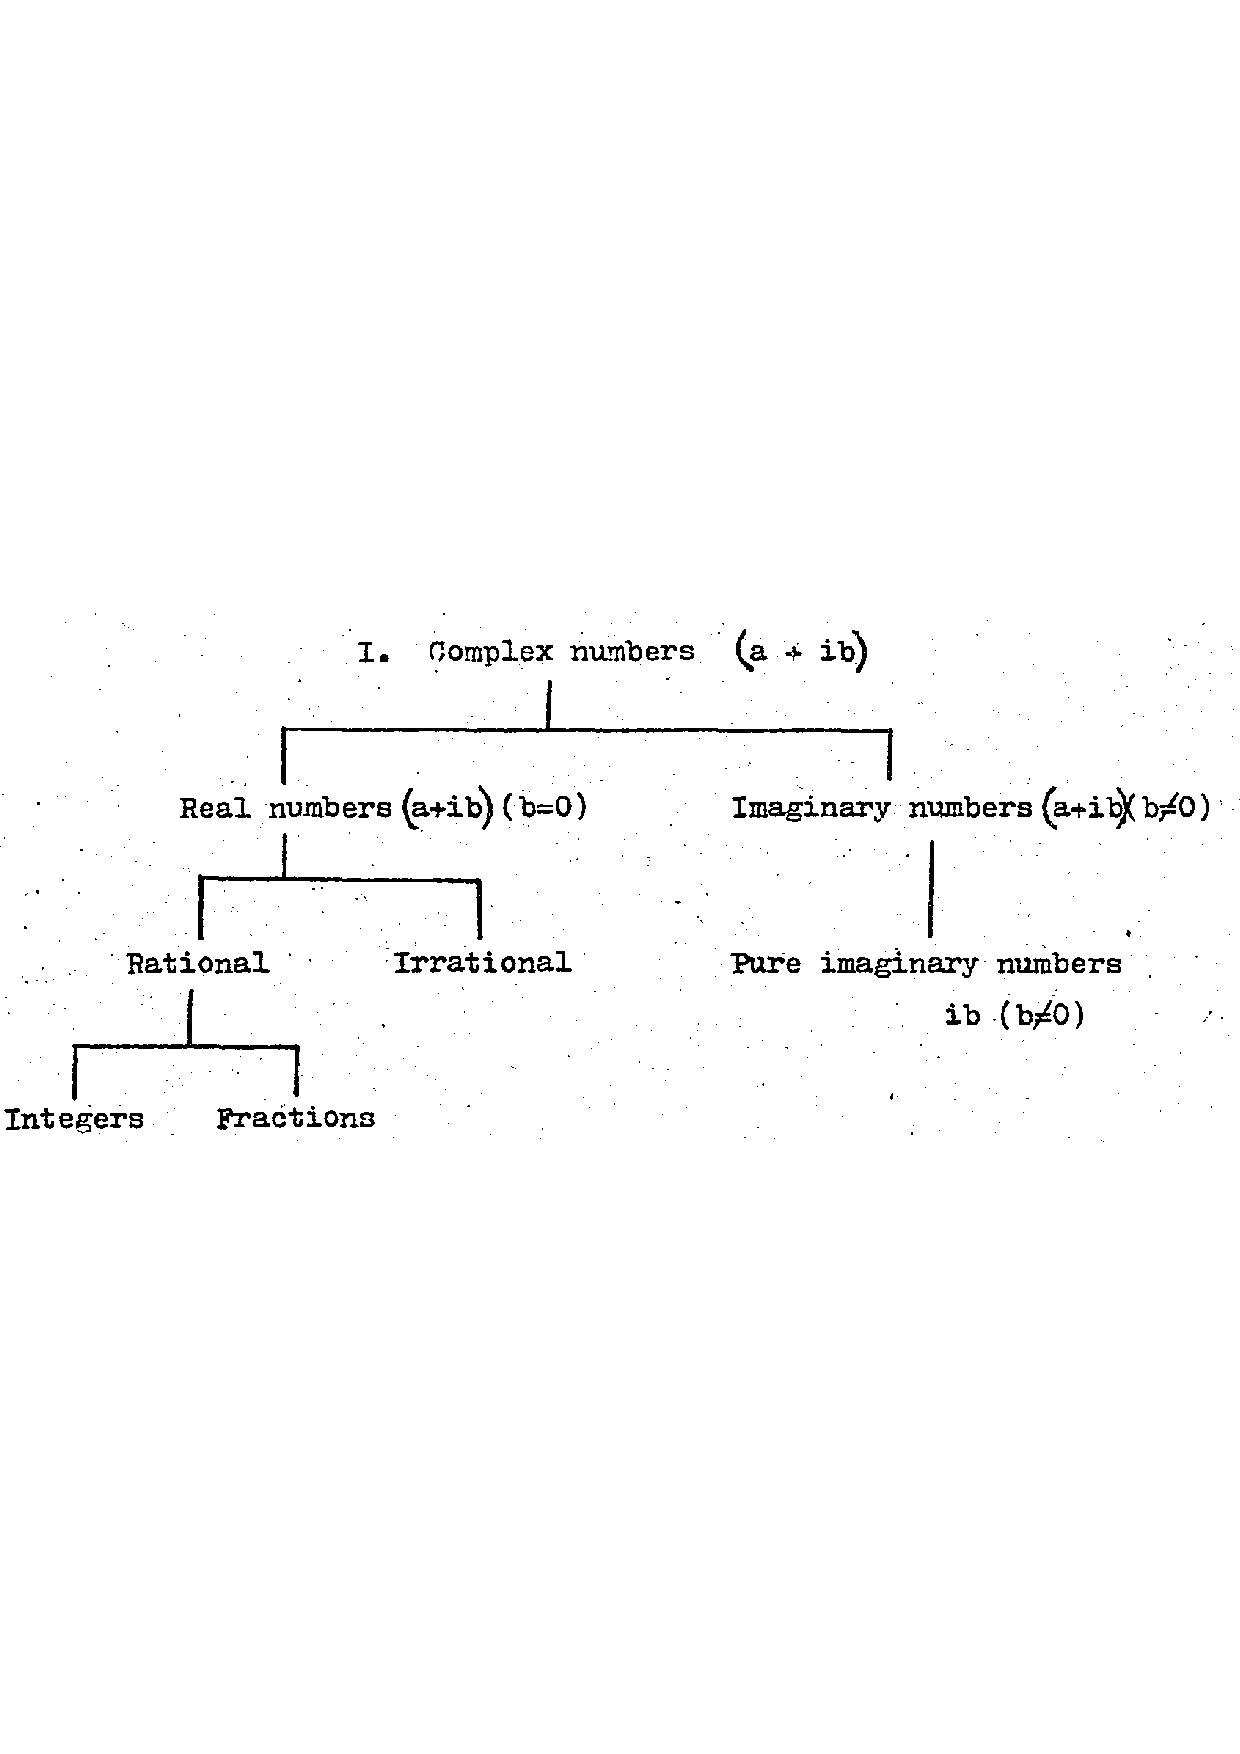
\includegraphics[width=0.9\textwidth]{images/SD-1-1p15A}
%	\caption{Classification of complex numbers}
%	\label{fig:classificationOfComplexNumbersA}
%\end{figure}

%\begin{center}
%\begin{tabular}{cc}
%\end{tabular}
%\end{center}

%\begin{exmp}
%\begin{hSolution}
%\end{hSolution}
%\end{exmp}

%\begin{hEnumerateAlpha}
%\end{hEnumerateAlpha}

%\begin{hEnumerateRoman}
%\end{hEnumerateRoman}

%$
%\begin{bmatrix}
%\end{bmatrix}
%$

%\frac{aaaa}{bbb}
%\frac{a_{n}}{b_{n}}
%\left( aaaa \right)
%\Longrightarrow

%\begin{multicols}{2}
%	bb
%\columnbreak
%	aa
%\end{multicols}
